\section{Support\-Disj Class Reference}
\label{class_support_disj}\index{SupportDisj@{SupportDisj}}
Class used to store additional informations in each node, here the support and the disjunction of the corresponding items.  


{\tt \#include $<$Support\-Disj.hpp$>$}

Inheritance diagram for Support\-Disj::\begin{figure}[H]
\begin{center}
\leavevmode
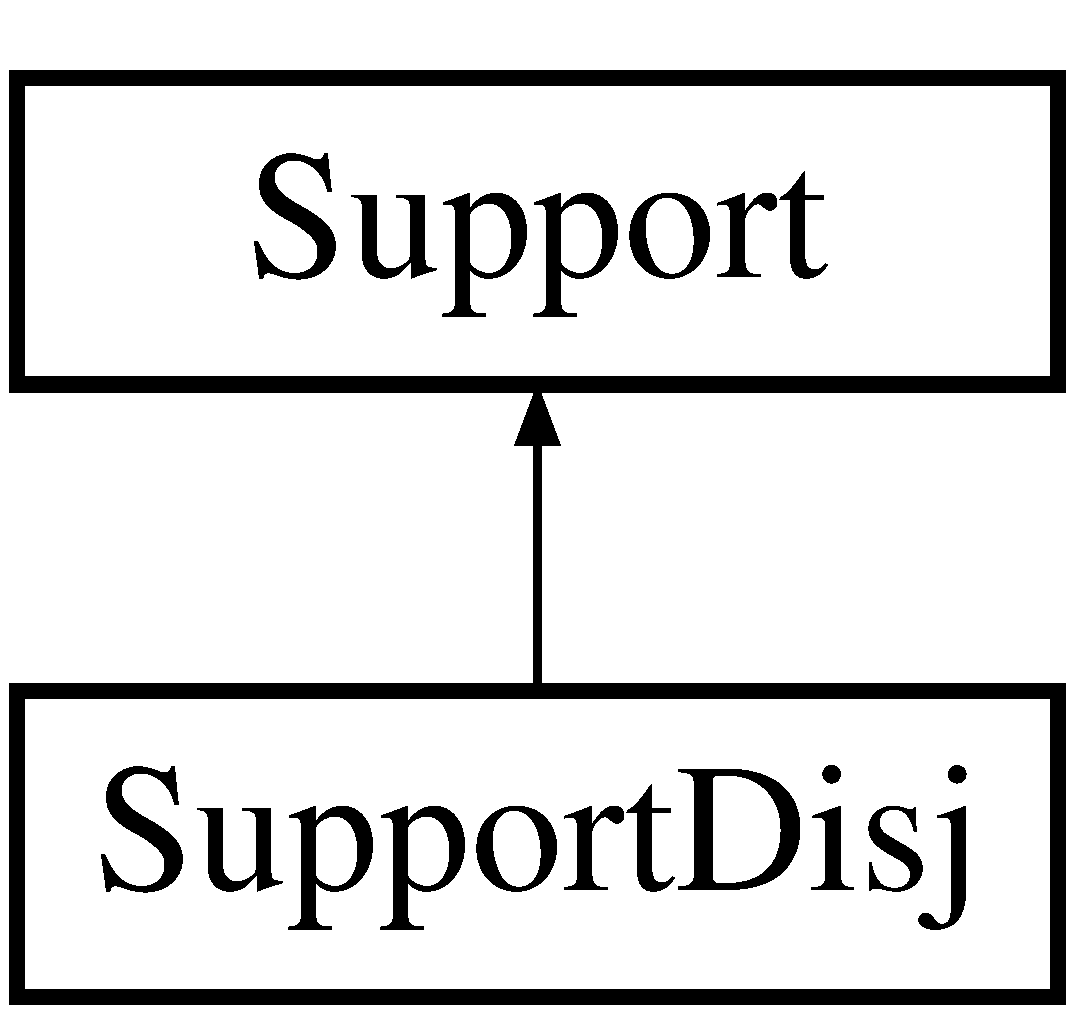
\includegraphics[height=2cm]{class_support_disj}
\end{center}
\end{figure}
\subsection*{Public Member Functions}
\begin{CompactItemize}
\item 
{\bf Support\-Disj} ()
\begin{CompactList}\small\item\em The constructor by deault, in cunjonction with the operator != to mark that an element is in a node. \item\end{CompactList}\end{CompactItemize}
\subsection*{Public Attributes}
\begin{CompactItemize}
\item 
int {\bf disj}\label{class_support_disj_ca1aa0fb612051f04e0ea48051fea157}

\begin{CompactList}\small\item\em store the disjunction of the corresponding itemset \item\end{CompactList}\end{CompactItemize}


\subsection{Detailed Description}
Class used to store additional informations in each node, here the support and the disjunction of the corresponding items. 

The disjunction is the number of transactions intersecting an itemset. 



\subsection{Constructor \& Destructor Documentation}
\index{SupportDisj@{Support\-Disj}!SupportDisj@{SupportDisj}}
\index{SupportDisj@{SupportDisj}!SupportDisj@{Support\-Disj}}
\subsubsection{\setlength{\rightskip}{0pt plus 5cm}Support\-Disj::Support\-Disj ()\hspace{0.3cm}{\tt  [inline]}}\label{class_support_disj_f55cb6b997d16ef0a60148b3091af369}


The constructor by deault, in cunjonction with the operator != to mark that an element is in a node. 

An element is in in the node is the {\bf Support}{\rm (p.\,\pageref{class_support})} of the current node is != of {\bf Support()}{\rm (p.\,\pageref{class_support_19bf40018bf3004487c65f7e68c9f65e})}. 

The documentation for this class was generated from the following file:\begin{CompactItemize}
\item 
F:/i\-Zi/problems/essential/Support\-Disj.hpp\end{CompactItemize}
